% template by Natalia Chernov for the University of Oldenburg

\documentclass[xcolor=table,9pt,aspectratio=169]{beamer}

\usepackage[utf8]{inputenc}

\usepackage{amsmath}
\usepackage{anyfontsize}
\usepackage[english,ngerman]{babel}
\usepackage[autostyle]{csquotes}
\usepackage{datetime}
\usepackage{helvet}
   \renewcommand{\familydefault}{\sfdefault}
\usepackage{hyperref}
   \urlstyle{same}
\usepackage{lipsum}
\usepackage{listings}
\usepackage{lmodern}
\usepackage{multicol}
\usepackage{multirow}
\usepackage{smartdiagram}
\usepackage{tikz}
\usepackage{xcolor}

\definecolor{uolblue}{RGB}{0,62,107}

\definecolor{blue1}{RGB}{0,78,159}
\definecolor{blue2}{RGB}{0,171,217}
\definecolor{blue3}{RGB}{91,197,242}
\definecolor{blue4}{RGB}{161,217,248}

\definecolor{green1}{RGB}{0,120,120}
\definecolor{green2}{RGB}{0,168,121}
\definecolor{green3}{RGB}{148,193,28}
\definecolor{green4}{RGB}{199,211,0}

\definecolor{orange1}{RGB}{213,59,10}
\definecolor{orange2}{RGB}{238,113,0}
\definecolor{orange3}{RGB}{243,145,0}
\definecolor{orange4}{RGB}{253,195,0}

\definecolor{gr}{RGB}{191,191,191}
\definecolor{grcode}{RGB}{190,190,190}

\lstdefinestyle{mystyle}{
   backgroundcolor=\color{grcode},
   commentstyle=\color{blue1},
   numberstyle=\tiny\color{blue1},
   basicstyle=\ttfamily\footnotesize,
   breakatwhitespace=false,
   breaklines=true,
   captionpos=b,
   keepspaces=true,
   numbers=left,
   numbersep=5pt,
   showspaces=false,
   showstringspaces=false,
   showtabs=false,
   tabsize=2
}

\setbeameroption{hide notes}
% \setbeameroption{show only notes}
% \setbeameroption{show notes on second screen=right}

\setbeamertemplate{frametitle}{\color{uolblue}\fontsize{12}{20}\selectfont{\insertframetitle}}

\pgfdeclareimage[width=0.145\paperwidth]{logo}{figures/logo_uol_negative}
\pgfdeclareimage[width=0.072\paperwidth]{logo_small}{figures/logo_uol_negative}

\defbeamertemplate*{background canvas}{default_page}
{%
\begin{tikzpicture}
   \useasboundingbox (0,0) rectangle (\the\paperwidth,\the\paperheight);
   \filldraw[fill=uolblue,fill opacity=1,draw=none] (0,0) rectangle (0.119\paperwidth,\the\paperheight);
   \filldraw[fill=blue2,fill opacity=1,draw=none] (0.119\paperwidth,0) -- (0.119\paperwidth,0.565\paperheight) arc (117.2:180:0.6\paperwidth) -- cycle;
   \pgftext[at=\pgfpoint{10}{\the\paperheight-11.5},left,top]{\pgfsetfillopacity{1}\pgfuseimage{logo_small}};
\end{tikzpicture}
}
\defbeamertemplate*{background canvas}{titlepage_image}
{
\begin{tikzpicture}
   \useasboundingbox (0,0) rectangle (\the\paperwidth,\the\paperheight);
   \filldraw[fill=uolblue,fill opacity=1,draw=none] (0,0) rectangle (\the\paperwidth,\the\paperheight);
   \filldraw[fill=blue2,fill opacity=1,draw=none] (\the\paperwidth,0) -- (\the\paperwidth,0.66\paperheight) arc (90:180:0.6\paperwidth) -- cycle;
   \pgftext[at=\pgfpoint{14}{\the\paperheight-17.5},left,top]{\pgfsetfillopacity{1}\pgfuseimage{logo}};
\end{tikzpicture}
}
\BeforeBeginEnvironment{frame}{%
   \setbeamertemplate{background canvas}[default_page]%
}
\makeatletter
\define@key{beamerframe}{titlepage_image}[true]{%
   \setbeamercovered{invisible}%
   \setbeamertemplate{background canvas}[titlepage_image]%
}
\makeatother%

\setbeamertemplate{footline}
{
   \leavevmode
   \hbox{
   \hspace*{.025\paperwidth}\begin{beamercolorbox}[wd=.094\paperwidth,ht=2.25ex,dp=1ex,left]{}
   ~

   \vspace*{.042\paperheight}
      \fontsize{4.4}{5.9}\selectfont\color{white}\textbf{Folie \insertframenumber}\newline\insertdate
   \vspace*{.026\paperheight}
   \end{beamercolorbox}
   \hspace*{.05\paperwidth}\begin{beamercolorbox}
   [wd=.79\paperwidth,ht=2.25ex,dp=1ex,left]{}
   ~

   \vspace*{.042\paperheight}
      \fontsize{4.4}{5.9}\selectfont\color{black}\textbf{Topics in the Cognitive Science of Morality}\newline\color{gray}\insertauthor~--~Fakultät IV, Institut für Philosophie
   \vspace*{.026\paperheight}
   \end{beamercolorbox}
   }
   \vskip0pt
}

\setbeamerfont{title}{size={\fontsize{22}{25}}}
\setbeamerfont{subtitle}{size={\fontsize{12}{14}}}
\setbeamerfont{author}{size={\fontsize{9}{11}}}
\setbeamerfont{date}{size={\fontsize{9}{11}}}
\setbeamercolor{title}{fg=white}
\setbeamercolor{subtitle}{fg=white}
\setbeamercolor{author}{fg=white}
\setbeamercolor{date}{fg=white}
\setbeamercolor{color_Logo-Platzhalter}{fg=white,bg=gray!40}

\defbeamertemplate*{title page}{customized}[1][]
{  \vspace*{20mm}
   \hspace*{-22.5mm}
   \begin{minipage}{\textwidth}
   \usebeamerfont{title}\usebeamercolor[fg]{title}\inserttitle\par
   \bigskip
   \usebeamerfont{subtitle}\usebeamercolor[fg]{subtitle}\insertsubtitle\par
   \bigskip
   \usebeamerfont{author}\usebeamercolor[fg]{author}\insertauthor\par
   \bigskip
   \usebeamerfont{date}\usebeamercolor[fg]{date}\insertdate\par
   \end{minipage}
}
\setbeamertemplate{navigation symbols}{}
\setbeamersize{text margin left=0.17\paperwidth,text margin right=0.04\paperwidth}

\title{Topics in the Cognitive Science\\of Morality}
\subtitle{Ringvorlesung}
\author{Alexander Max Bauer}
\date{WiSe 2026/2027}
% \date{\renewcommand{\dateseparator}{.}\ddmmyyyydate\today}
\usepackage{enumitem}
\def\labelitemi{--}
\def\labelitemii{--}
\def\labelitemiii{--}

\begin{document}
{
\setbeamertemplate{footline}{}
\begin{frame}[titlepage_image]
   \maketitle
\end{frame}
}


%%%%%%%%%%%%%%%%%%%%%%%%
% FOLIE 2 – GLIEDERUNG %
%%%%%%%%%%%%%%%%%%%%%%%%
\begin{frame}{\vspace*{10mm}Gliederung}
\begin{itemize}
   \item[1] Einführung und Organisatorisches
   \begin{itemize}
      \item Lehrende
      \item Ankündigungstext, Format, Plattformen
      \item Sprache, Sprechstunden, Zusatzinformationen
      \item Seminarstruktur
      \item Modulzuordnung und Prüfungsformen
      \item Ablaufplan
   \end{itemize}
   \item[2] Literatur
\end{itemize}
\end{frame}


%%%%%%%%%%%%%%%%%%%%%%%%
% FOLIE 3 - EINFÜHRUNG %
%%%%%%%%%%%%%%%%%%%%%%%%
\begin{frame}
\begin{overlayarea}{\textwidth}{0.81\paperheight}{
   \vspace*{11mm}
   \usebeamerfont{title}\textcolor{uolblue}
   {1\hspace*{1em}Einführung und Organisatorisches}
}
\end{overlayarea}
\end{frame}


%%%%%%%%%%%
% FOLIE 4 %
%%%%%%%%%%%
\begin{frame}{\vspace*{10mm}1\hspace*{1em}Einführung und Organisatorisches}
\textbf{Lehrende}\\
\begin{multicols}{2}
   \begin{center}
      \frame{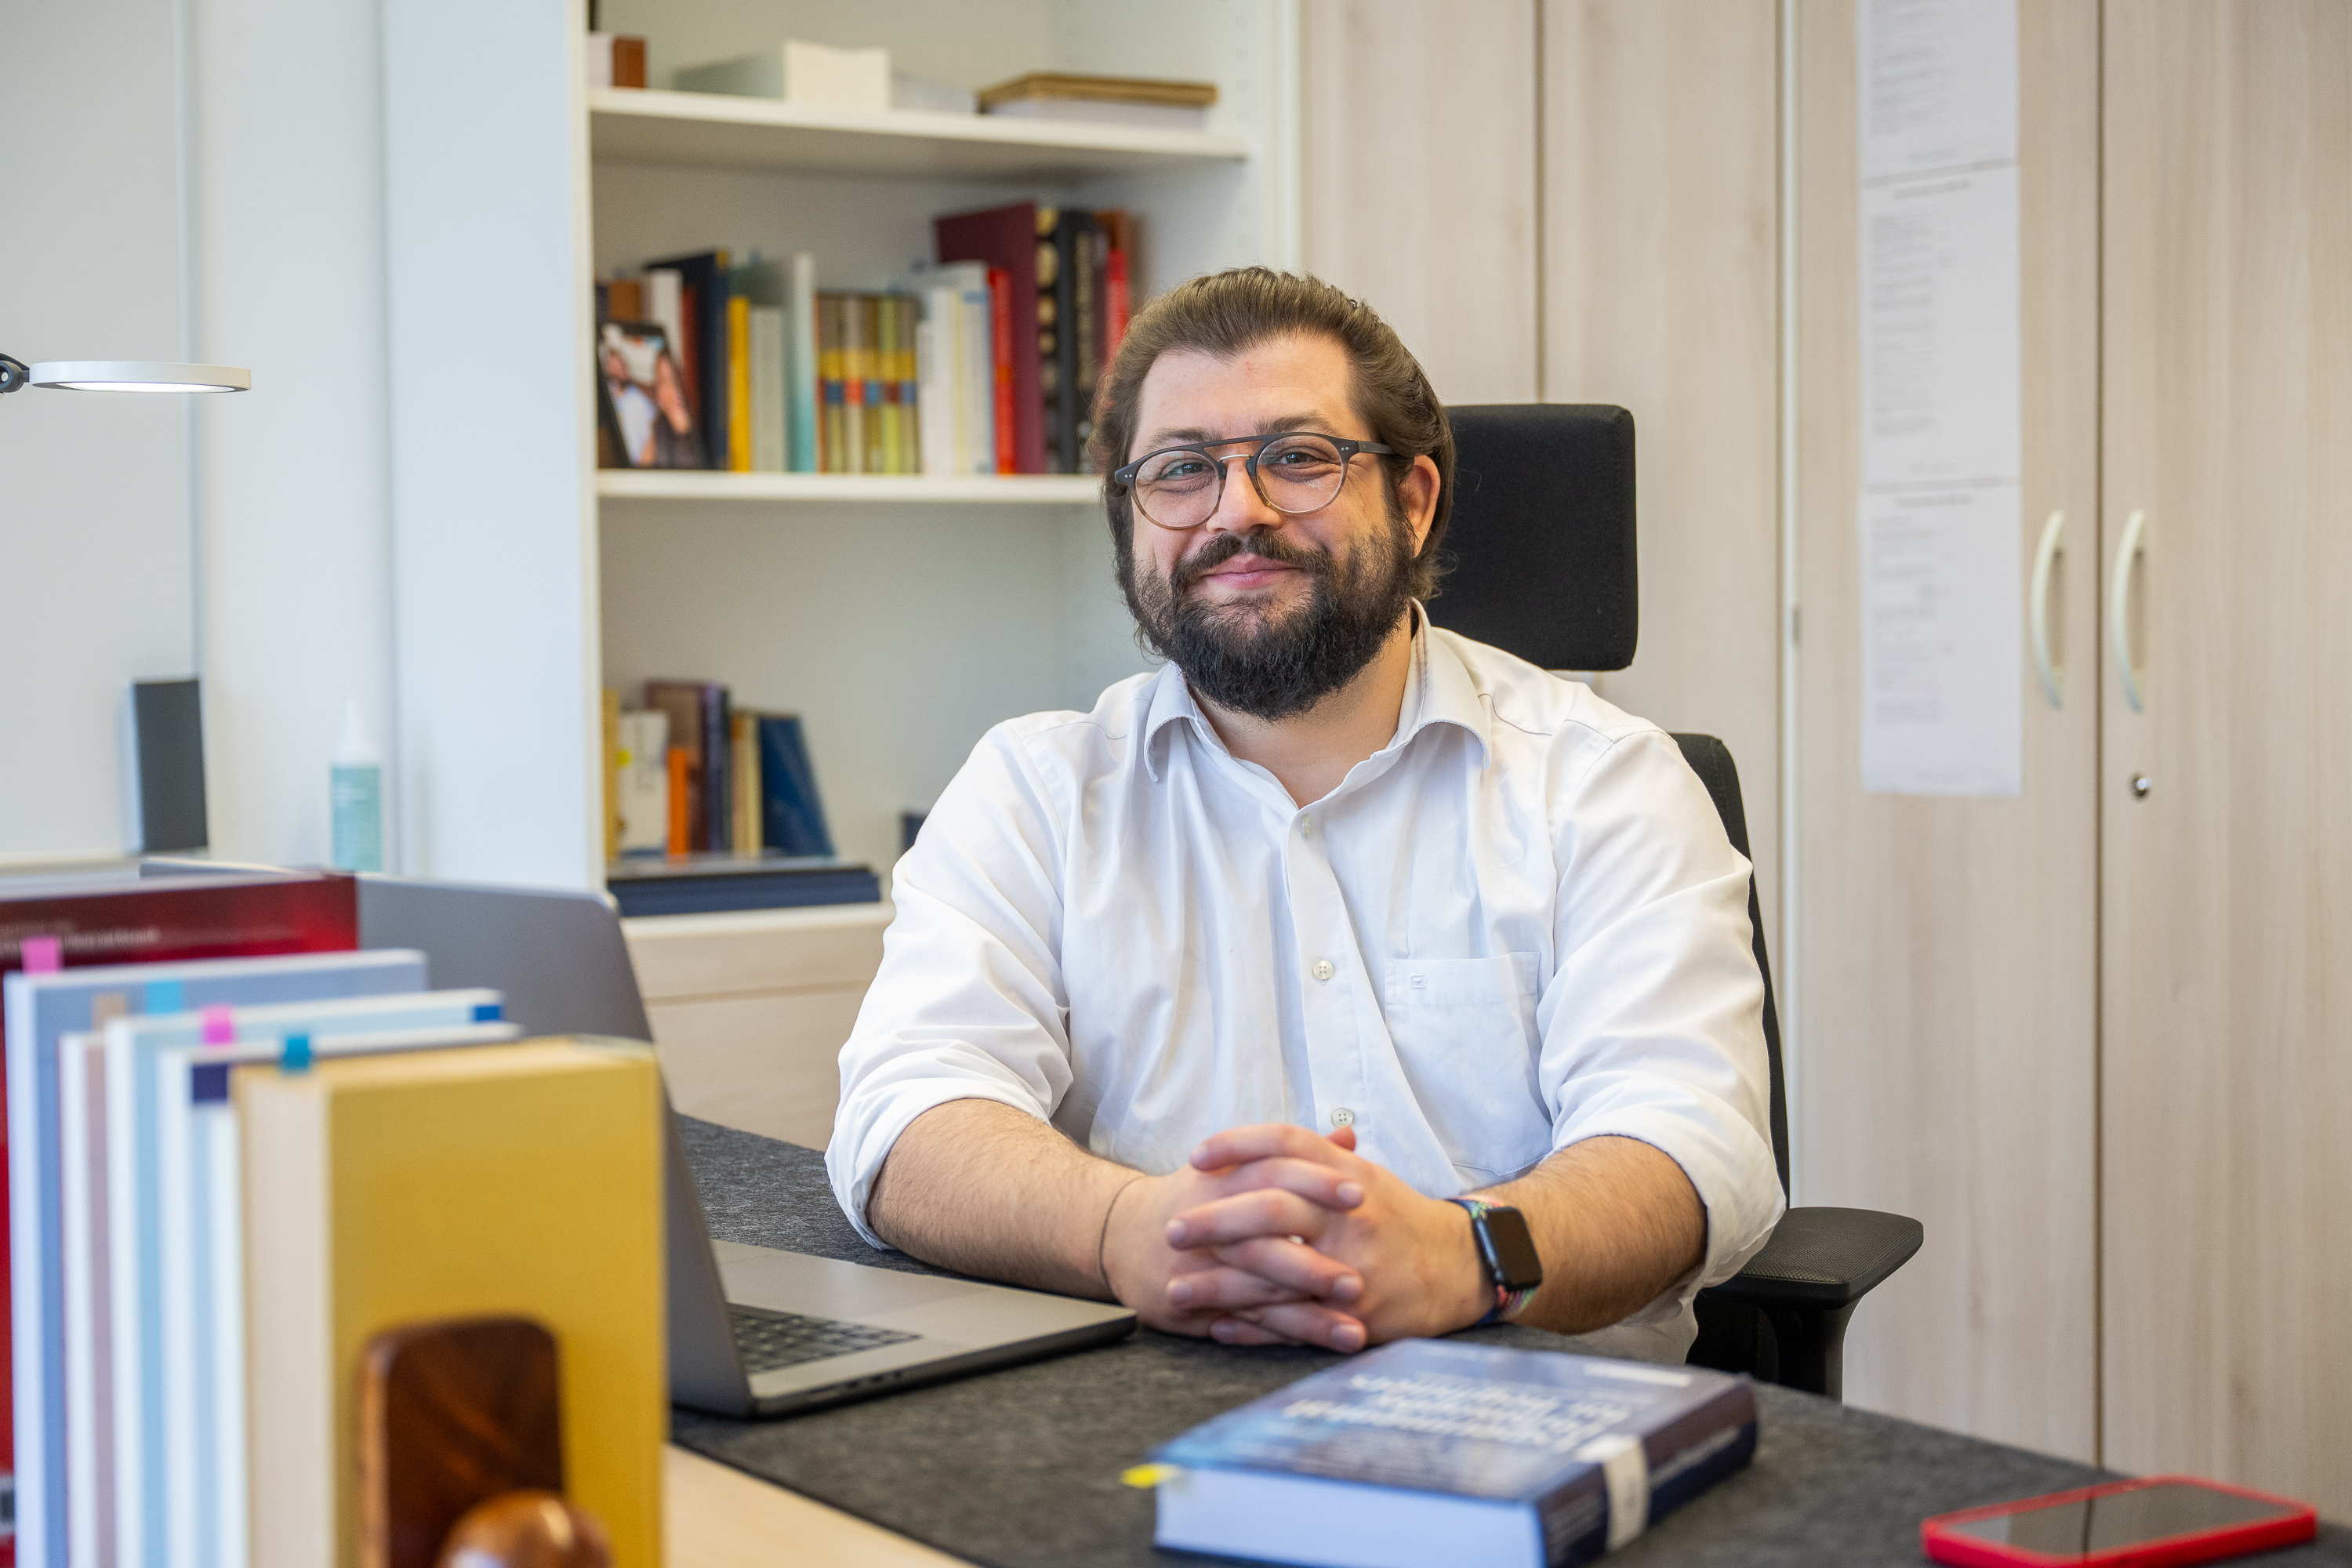
\includegraphics[height=0.35\textheight]{figures/bauer.jpg}}\\
      Alexander Max Bauer,\\
      Universität Oldenburg\\
      \textcolor{gray}{(Foto: Daniel Schmidt)}\\
      \frame{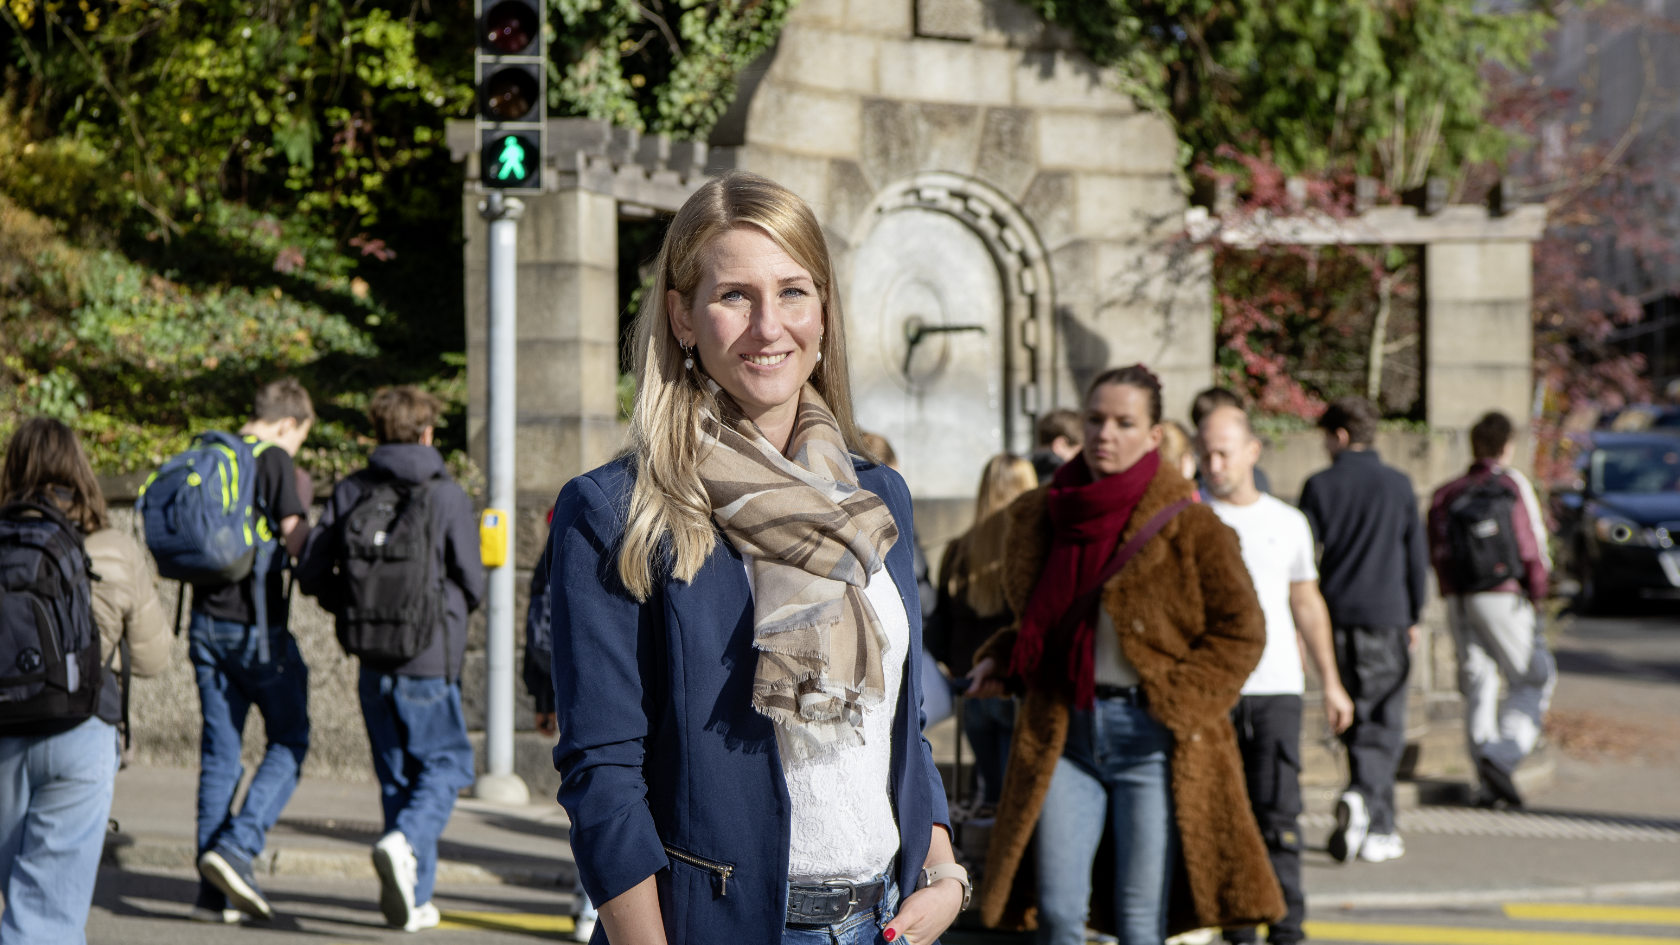
\includegraphics[height=0.35\textheight]{figures/willemsen.jpg}}\\
      Pascale Willemsen,\\
      Universität Zürich\\
      \textcolor{gray}{(Foto: Ursula Meisser)}
   \end{center}
\end{multicols}
\end{frame}


%%%%%%%%%%%
% FOLIE 5 %
%%%%%%%%%%%
\begin{frame}{\vspace*{10mm}1\hspace*{1em}Einführung und Organisatorisches}
\textbf{Ankündigungstext:} Diese Ringvorlesung bietet einen Einblick in aktuelle Debatten und interdisziplinäre Forschungsansätze an der Schnittstelle von Kognitionswissenschaft und Moral.
Das Modul folgt grob einem zweiwöchentlichen Rhythmus:
In jeder zweiten Woche präsentieren führende internationale Expert:innen aus der Philosophie, Linguistik und Psychologie ihre aktuelle Forschung.
Die jeweils dazwischenliegenden Wochen dienen der inhaltlichen Vorbereitung auf diese Gastvorträge.

\medskip
\textbf{Format:} Gastvorträge finden online statt, die Vorbereitung findet in Präsenz statt.

\medskip
\textbf{Plattformen:} Der Kooperation mit Zürich wegen findet diese Veranstaltung online mit Teams statt mit Big Blue Button statt. Literatur wird auf Stud.IP zur Verfügung gestellt.
\end{frame}


%%%%%%%%%%%
% FOLIE 6 %
%%%%%%%%%%%
\begin{frame}{\vspace*{10mm}1\hspace*{1em}Einführung und Organisatorisches}
\textbf{Sprache:} Die Gastvorträge finden teilweise auf Englisch und teilweise auf Deutsch statt.
Die Sprache in den anschließenden Diskussionen richtet sich nach der Vortragssprache.

\medskip
\textbf{Sprechstunden:} Kurze Fragen können vor und nach der Veranstaltung geklärt werden. Für umfangreichere Fragen können Sprechstunden vereinbart werden.

\medskip
\textbf{Zusatzinformation:} Die Ringvorlesung findet als gemeinsame Veranstaltung mit der Universität Zürich statt.
Das Semester in Oldenburg beginnt und endet später als dort.
Studierende haben aber die Möglichkeit, auch die Vorträge vor dem Semesterbeginn in Oldenburg zu besuchen.
\end{frame}


%%%%%%%%%%%
% FOLIE 7 %
%%%%%%%%%%%
\begin{frame}{\vspace*{10mm}1\hspace*{1em}Einführung und Organisatorisches}
\textbf{Seminarstruktur}\\
\begin{flushleft}
   \smartdiagramset{uniform sequence color=true,
   sequence item uniform color=blue2,
   sequence item border color=white,
   sequence item font size=\footnotesize,
   sequence item text color=white,
   sequence item height=1.5cm,
   sequence item width=1.8cm
   }
   \smartdiagram[sequence diagram]{Vorbereitung (Präsenz), Vortrag\\(Online), $\ldots$}
\end{flushleft}
\end{frame}


%%%%%%%%%%%
% FOLIE 8 %
%%%%%%%%%%%
\begin{frame}{\vspace*{10mm}1\hspace*{1em}Einführung und Organisatorisches}
\textbf{Modulzuordnung und Prüfungsformen}\\
\begin{itemize}
   \item \textbf{phi321:} Praktische Philosophie und ihre Konsequenzen für die Gesellschaft
   \item \textbf{phi331:} Theoretische Philosophie und ihre Konsequenzen für die Grundlagen der Wissenschaften
   \begin{itemize}
      \item Hausarbeit \textcolor{gray}{(16\,--\,18 Seiten)}
      \item Referat \textcolor{gray}{(30\,--\,35 Minuten)} mit schriftlicher Ausarbeitung \textcolor{gray}{(10\,--\,12 Seiten)}
      \item Mündliche Prüfung \textcolor{gray}{(25\,--\,30 Minuten)}
   \end{itemize}
   \item \textbf{phi340:} Praktische Philosophie -- Ethik, Recht, Gesellschaft
   \begin{itemize}
      \item Hausarbeit \textcolor{gray}{(10\,--\,12 Seiten)}
      \item Referat \textcolor{gray}{(20\,--\,25 Minuten)} mit schriftlicher Ausarbeitung \textcolor{gray}{(6\,--\,8 Seiten)}
      \item Mündliche Prüfung \textcolor{gray}{(15\,--\,20 Minuten)}
   \end{itemize}
\end{itemize}
\end{frame}


%%%%%%%%%%%
% FOLIE 9 %
%%%%%%%%%%%
\begin{frame}{\vspace*{10mm}1\hspace*{1em}Einführung und Organisatorisches}
\textbf{Ablaufplan (1/2)}\\
\smallskip
\begin{tabular}[h]{llll}
   \arrayrulecolor{blue2}\hline
   Datum        & \multicolumn{2}{c}{Universität}   & Inhalt                                             \\
   \hline
   16.09.2026   & Zürich   &                        & Einführung und Organisatorisches (Zürich)          \\
   23.09.2026   & Zürich   &                        & Künstliche Intelligenz und Verantwortung           \\
                &          &                        & \textcolor{gray}{(Hyungrae Noh und Dongwoo Kim)}   \\
   30.09.2026   & Zürich   &                        & Vorbereitung                                       \\
   07.10.2026   & Zürich   &                        & Moralischer Objektivismus                          \\
                &          &                        & \textcolor{gray}{(Miklós Kürthy)}                  \\
   14.10.2026   & Zürich   & Oldenburg              & Einführung und Organisatorisches (Oldenburg)       \\
   21.10.2026   & Zürich   & Oldenburg              & Moralische Pflichten gegenüber Toten               \\
                &          &                        & \textcolor{gray}{(Joanna Demarree-Cotton)}         \\
   28.10.2026   & Zürich   & Oldenburg              & Moralische Anforderungen an Überzeugungen          \\
                &          &                        & \textcolor{gray}{(Kevin Reuter)}                   \\
   04.11.2026   & Zürich   & Oldenburg              & Feministische Philosophie                          \\
                &          &                        & \textcolor{gray}{(Sebastian Bernhard)}             \\
   \hline
\end{tabular}
\end{frame}


%%%%%%%%%%%%
% FOLIE 10 %
%%%%%%%%%%%%
\begin{frame}{\vspace*{10mm}1\hspace*{1em}Einführung und Organisatorisches}
\textbf{Ablaufplan (2/2)}\\
\smallskip
\begin{tabular}[h]{llll}
   \arrayrulecolor{blue2}\hline
   Datum        & \multicolumn{2}{c}{Universität}   & Inhalt                                  \\
   \hline
   11.11.2026   & Zürich   & Oldenburg              & Vorbereitung                            \\
   18.11.2026   & Zürich   & Oldenburg              & Leihmutterschaft                        \\
                &          &                        & \textcolor{gray}{(Pascale Willemsen)}   \\
   25.11.2026   & Zürich   & Oldenburg              & Vorbereitung                            \\
   02.12.2026   & Zürich   & Oldenburg              & Sprache in der Politik                  \\
                &          &                        & \textcolor{gray}{(Nicole Gotzner)}      \\
   09.12.2026   & Zürich   & Oldenburg              &                                         \\
   16.12.2026   &          & Oldenburg              & Vorbereitung                            \\
   13.01.2027   &          & Oldenburg              & Trauer und personale Identität          \\
                &          &                        & \textcolor{gray}{(Vilius Dranseika)}    \\
   20.01.2027   &          & Oldenburg              &                                         \\
   27.01.2027   &          & Oldenburg              & Abschluss                               \\
   \hline
\end{tabular}
\end{frame}


%%%%%%%%%%%%%%%%%%%%%%%%
% FOLIE 11 - LITERATUR %
%%%%%%%%%%%%%%%%%%%%%%%%
\begin{frame}
\begin{overlayarea}{\textwidth}{0.81\paperheight}{
   \vspace*{11mm}
   \usebeamerfont{title}\textcolor{uolblue}
   {2\hspace*{1em}Literatur}
}
\end{overlayarea}
\end{frame}


%%%%%%%%%%%%
% FOLIE 12 %
%%%%%%%%%%%%
\begin{frame}{\vspace*{10mm}2\hspace*{1em}Literatur}
23.09.2026

\vspace{1em}
Hyungrae Noh (Korea Advanced Institute of Science \& Technology, Südkorea)

\textit{Two Senses of Responsibility -- Retribution, Rule Violation, and AI}

\vspace{1em}
\textbf{Grundlegende Literatur}
{\footnotesize
\begin{itemize}[label=,leftmargin=2em,itemindent=-2em]
   \item Noh, Hyungrae (in Vorbereitung): \enquote{AI Is Morally Responsible, Just Not in the Retributive Sense. Evidence From Folk Judgment}.
\end{itemize}
}

\vspace{1em}
\textbf{Weiterführende Literatur}

{\footnotesize
\begin{itemize}[label=,leftmargin=2em,itemindent=-2em]
   \item Berman, Mitchell (2023): \enquote{Blameworthiness, Desert, and Luck}, \textit{Noûs} 57~(2), S.~370--390.
   \item Kneer, Markus, und Markus Christen (2024): \enquote{Responsibility Gaps and Retributive Dispositions. Evidence From the US, Japan and Germany}, \textit{Science and Engineering Ethics} 30, 51.
   \item Malle, Bertram, Steve Guglielmo und Andrew Monroe (2014): \enquote{A Theory of Blame}, \textit{Psychological Inquiry} 25~(2), S.~147--186.
\end{itemize}
}
\end{frame}


%%%%%%%%%%%%
% FOLIE 13 %
%%%%%%%%%%%%
\begin{frame}{\vspace*{10mm}2\hspace*{1em}Literatur}
23.09.2026

\vspace{1em}
Dongwoo Kim (Korea Advanced Institute of Science \& Technology, Südkorea)

\textit{The Structure of Folk Responsibility Judgments for AI-Mediated Harms}

\vspace{1em}
\textbf{Grundlegende Literatur}
{\footnotesize
\begin{itemize}[label=,leftmargin=2em,itemindent=-2em]
   \item Noh, Hyungrae, Garam Kim, Jiyoung Park, Ijin Kim und Dongwoo Kim (in Vorbereitung): \enquote{Who's Responsible, and in What Ways? The Structure of Folk Responsibility Judgments for AI-Mediated Harms Across Special- and General-Purpose Systems}.
\end{itemize}
}

\vspace{1em}
\textbf{Weiterführende Literatur}

{\footnotesize
\begin{itemize}[label=,leftmargin=2em,itemindent=-2em]
   \item Danaher, John (2016): \enquote{Robots, Law and the Retribution Gap}, \textit{Ethics and Information Technology} 18, S.~299--309.
   \item Floridi, Luciano, und Jeffrey Sanders (2004): \enquote{On the Morality of Artificial Agents}, \textit{Minds and Machines} 14, S.~349--379.
   \item Matthias, Andreas(2004): \enquote{The Responsibility Gap. Ascribing Responsibility for the Actions of Learning Automata}, \textit{Ethics and Information Technology} 6, S.~175--183.
\end{itemize}
}
\end{frame}


\end{document}
